\documentclass{article}
\usepackage[utf8]{inputenc}
\usepackage[russian]{babel}
\usepackage{seqsplit}
\usepackage{graphicx}
\usepackage{color,soul}
\usepackage{systeme}
\usepackage{amsmath}

\title{Time Series}
\author{andreisaw}
\date{March 2019}

\begin{document}

\maketitle

\section{Введение}
Временной ряд: в файле ``input.csv''. Количество наблюдений $N=200$

Нарисуем реализацию

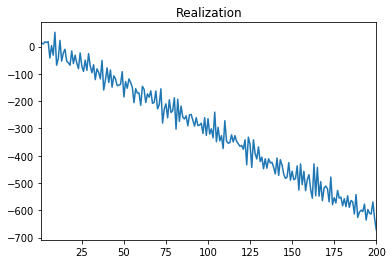
\includegraphics[width=\linewidth]{image.png}
Модель ВР \begin{gather*}
    X_t = \mu + bt +\alpha_1X_{t-1} + \ldots + \alpha_p X_{t-p} + \varepsilon_t,\\
    X_t = \mu +bt +\sum_{j=1}^{p}\alpha_jX_{t-1} + (X_{t-1} - X_{t-2})(-\alpha_2-\ldots -\alpha_p)\\
    = \mu + bt +\sum_{j=1}^{p}\alpha_jX_{t-1} + \theta_1\Delta X_{t-1} + \ldots + \theta_p\Delta X_{t-p} +\varepsilon_t,\\ \theta= -\alpha_{j+1}-\ldots-\alpha_p,\\
    \Delta X_t=X_t - X_{t-1}=\mu+bt+(\sum_{j=1}^{p}\alpha_j-1)X_{t-1}+\sum_{j=1}^{p}\theta_j\Delta X_{t-j}+\varepsilon_t
\end{gather*}
\begin{gather}
    \Delta X_t = \mu +bt + \gamma X_{t-1} + \sum_{j=1}^{p}\theta_j \Delta X_{t-j} +\varepsilon_t
\end{gather}
Где 
\begin{gather*}
    \varepsilon_t \sim WN(0,\sigma^2)\\
    p <= N^{1/3}
\end{gather*}

Нужно вычислить какое количество запаздываний являются значимыми и уточнить формулу (1). Количество запаздываний $p <= 5.8$. Для этого посчитаем $p-value$ на уровне значимости $\alpha=0.05$ для коэффициентов $\alpha_1,\ldots,\alpha_5$ модели с $p=5$ запаздываниями.

\begin{gather*}
    \alpha_1=0.000,\\
    \alpha_2=0.005,\\
    \alpha_3=0.421,\\
    \alpha_4=0.558,\\
    \alpha_5=0.855
\end{gather*}
Таким образом, значимые только $\alpha_1, \alpha_2$. Модели принимает вид:
\begin{gather}
        \Delta X_t = \mu +bt + \gamma X_{t-1} + \theta_1 \Delta X_{t-1} +\varepsilon_t
\end{gather}
Используем Процедуру Dolado-Jenkinson-Sosvilla-Rivero для того, чтобы определить к какому типу относится ВР - $TSP$ или $DSP$. Процедура состоит из пяти шагов.

\textit{Шаг1.} Проверить гипотезу $H_0: \sum_{j=1}^{p}\alpha_j-1=\gamma = 0$ против альтернативной гипотезы $H_A: \gamma < 0$, с помощью ADF-статистики $DF_tr(\alpha=0.05)$, если $H_0$ отвергается, то $\gamma < 0$ и проверяемый ВР можно отнести к типу TSP. 
\begin{gather*}
    \hat{DF}_{tr} = \frac{\hat{\gamma}}{S(\hat{\gamma})}
\end{gather*}
Гипотеза отвергается на уровне значимости $\alpha=0.05$, если $ \hat{DF}_{tr}<DF_tr(\alpha=0.05)$\newline

ADF Statistic: \hl{-10.485569}

p-value: 0.000000

usedlags: 2

Critical Values:

	1\%: -4.005 
	
	5\%: \hl{-3.433}
	
	10\%: -3.140\newline

Поскольку $-10.485569 <-3.433 $ то необходимо отвергнуть $H_0$. И \textbf{временной ряд - типа TSP}.\newpage

\section{Оценка тренда}
Рассмотрим аддитивную модель ВР: $x_t = d_t +\varepsilon_t$, $t=1,\ldots,n$\newline
Необходимо оценить детерминированную состовляющую ряда. Для этого нужно использовать Метод Наименьших Квадратов (МНК).\newline
Пусть тренд $f(t) = \theta_0 + \theta_1t$ - линейный тренд.\newline \newline
И тогда \begin{gather*}
    \hat{\theta_0} = \bar{y} - \hat{\theta_1} \bar{x},\\ 
    \hat{\theta_1} = \frac{\sum_{i=1}^{n}{(x_i - \bar{x})(y_i - \bar{y})}}{\sum_{i=1}^{n}{(x_i - \bar{x})^2}}
\end{gather*}
По расчетам $\hat{\theta_0} = 19.70$, $\hat{\theta_1} = -3.227509$

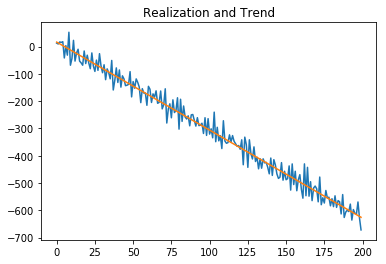
\includegraphics[width=\linewidth]{trend.png}\newpage

\section{Детрендирование ряда}

Для того чтобы детренедировать ВР, необходимо посчитать $X_i - (\hat{\theta_0} + \hat{\theta_1}i)$\newline
Детрендированный ряд находится в файле ``output.csv''\newline\newline

Нарисуем  \newline
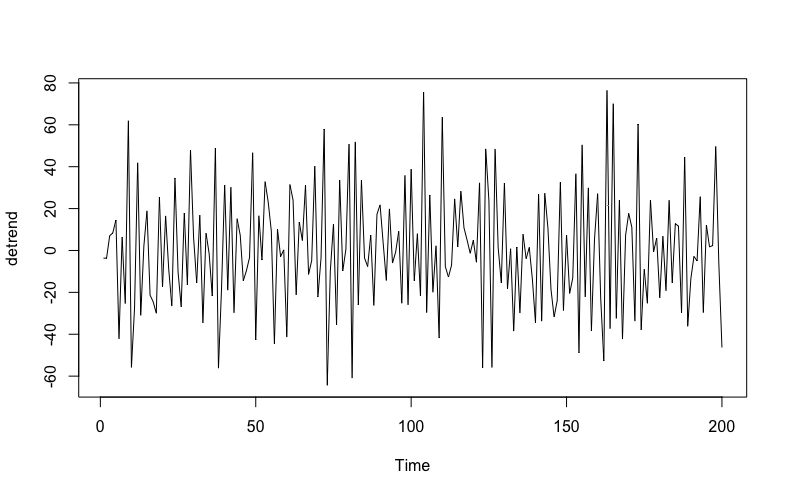
\includegraphics[width=\linewidth]{Rplot.png}\newpage

\section{Идентификация случайно составляющей ряда}
Необходимо построить выборочные Автокорреляционную и Частную Автокорреляционную функции для $X_{notrend}$, и опираясь на характерные свойства этих функций, выбрать наиболее вероятную модель.\newline
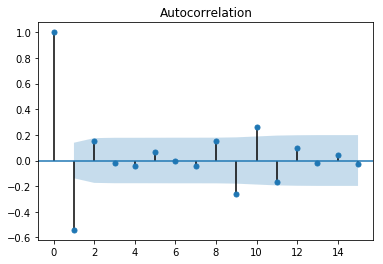
\includegraphics[width=\linewidth]{pacf_acf.png}\newline
$\rho = \seqsplit{%
1.000, -0.541, 0.154, -0.021, -0.046, 0.064, -0.000, -0.045, 0.151, -0.258, 0.261, -0.166, 0.100, -0.019, 0.045, -0.029, 0.030, -0.058, 0.114, -0.187, 0.132, -0.014, -0.021, -0.005, -0.023, 0.031, 0.040, -0.102, 0.118, -0.062, 0.005, -0.067, 0.016, 0.089, -0.139, 0.134, -0.072, -0.062, 0.129, -0.104, 0.119}$\newline
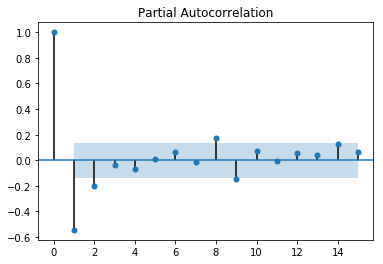
\includegraphics[width=\linewidth]{pacg.png}\newline
$\phi = \seqsplit{%
1.000, -0.544, -0.199, -0.040, -0.071, 0.007, 0.066, -0.012, 0.170, -0.144, 0.074, -0.004, 0.053, 0.038, 0.129, 0.068, 0.048, -0.002, 0.049, -0.118, -0.099, 0.050, 0.001, -0.025, -0.090, 0.004, 0.052, -0.051, -0.026, 0.066, 0.012, -0.162, -0.135, 0.119, -0.082, 0.062, 0.021, -0.069, 0.042, -0.018, 0.135}$\newline\newline

Асимптотическое распредение выборочной ЧАКФ $\hat{\phi}(h)$ модели $AR(p)$ имеет гауссовское распределение начиная с $p+1$ лага ($h>p$), с дисперсией 
\begin{gather*}
    Var(\hat{\phi}(h))\sim\frac{1}{n}
\end{gather*}
Т.е. с вероятностью 0.95 попадает в доверительный интервал $[-\frac{1.96}{\sqrt{n}}; \frac{1.96}{\sqrt{n}}]$\newline
Если $\hat{\phi}(h)$ для $h>p$ незначимы, то предполагаем, что модель - $AR(p)$\newline\newline

Асимптотическое распредление выборочной АКФ $\hat{\rho}(h)$ модели $MA(q)$ имеет гауссовское распределение начиная с $q+1$ лага ($h>q$), с дисперсией 
\begin{gather*}
    Var(\hat{\rho}(h))=\frac{1}{n}(1+2\sum_{k=1}^{q}\rho^2(k))
\end{gather*}
В общем случае, если $\hat{\rho}(h)$ для $h>p$ незначимы, то предполагаем, что модель - $MA(p)$\newline\newline

Рассмотрев график выборочной ЧАКФ, можно сделать преположение, что искомая модель - AR(2), судя по количеству значимых $\phi(h)$  - значения лагов 1,2,8,9. Однако, следует рассмотреть также модель ARMA(1,1).\newpage

\section{Оценка параметров модели}
\subsection{AR(2)}

Модель авторегрессии порядка $p$ представляет собой
\begin{gather*}
    x_n = \varepsilon_n + \sum_{j=1}^{p}\alpha_jx_{n-j}
\end{gather*}

Параметры для оценки: $\alpha_1,\ldots,\alpha_p$. Для оценки параметров AR модели необходимо составить уравнения Юла-Уокера.\newline

\left\{\begin{array}{l}{\rho(1)=\alpha_{1}+\alpha_{2} \rho(1)+\cdots+\alpha_{p} \rho(p-1)} \\ {\rho(2)=\alpha_{1} \rho(2)+\alpha_{2}+\cdots+\alpha_{p} \rho(p-2)} \\ {\ldots \ldots \ldots \ldots \ldots \ldots \ldots\\ {\rho(p)=\alpha_{1} \rho(p-1)+\alpha_{2} \rho(p-2)+\cdots+\alpha_{p}}\end{array}\right.\\

И тогда $\rho_p=R_p\alpha$ или $\alpha = R_p^{-1}\rho_p$, где $\alpha$  -  вектор искомых параметров модели AR.

Для $p=2$: 
\begin{gather*}
    x_n = \varepsilon_n + \alpha_1x_{n-1} + \alpha_2x_{n-2}\\
    \alpha = R_2^{-1}\rho_2,\\
    R_2^{-1} = \frac{1}{1-\rho^2(1)}
    \begin{bmatrix} 
        1 & -\rho(1) \\ -\rho(1) & 1
    \end{bmatrix},\\
    \rho_2 = \begin{pmatrix} \rho(1) \\ \rho(2) \end{pmatrix},
\end{gather*}
По расчетам: \newline
\begin{gather*}
    \hat{\alpha} = \begin{pmatrix}-0.647\\-0.196 \end{pmatrix}
\end{gather*}

\subsection{ARMA(1,1)}

Модель авторегрессии-скользящего среднего порядка $(p,q)$ представляет собой
\begin{gather*}
    x_n -\sum_{j=1}^{p}\alpha_jx_{n-j} = \varepsilon_n +\sum_{j=1}^{q}\beta_{j}\varepsilon_{n-j}
\end{gather*}

Для $p=1,q=1$: 
\begin{gather*}
    x_n -\alpha_1x_{n-1} = \varepsilon_n +\beta_{1}\varepsilon_{n-1}
\end{gather*}

Параметры для оценки: $\alpha_1,\beta_1$

Для оценки параметров $\alpha$ и $\beta$ модели ARMA необходимо решить систему уравнений:\newline

\left\{\begin{array}{l}{\rho_{X}(1)=\frac{(\alpha+\beta)(1+\alpha \beta)}{1+\beta^{2}+2 \alpha \beta}} \\ {\rho_{X}(2)=\frac{\alpha(\alpha+\beta)(1+\alpha \beta)}{1+\beta^{2}+2 \alpha \beta}}\end{array}\right.\\

По подсчетам: 
\begin{gather*}
    \hat{\alpha} = -0.285\\
    \hat{\beta} = 0.3764
\end{gather*}\newpage

\section{Оценка адекватности модели}
\subsection{Контроль качества}

Для оценки качества модели будут использоваться информационные критериии Акаике(AIC) и Шварца(BIC). Информационные критерии необходимо для того, чтобы предотвратить переобучение с помощью функции потерь для каждого дополнительного парметра в модели.\newline
\begin{gather*}
    AIC = \ln\hat{\sigma}^2+\frac{2(p+q)}{n}\\
    BIC = \ln\hat{\sigma}^2 + (p+q)\frac{\ln n}{n}
\end{gather*}
Для $AR(2)$ модели:
\begin{gather*}
    AIC=1843.4 \\ BIC=1856.59
\end{gather*}
Для $ARMA(1,1)$ модели:
\begin{gather*}
    AIC=1843.19 \\ BIC=1856.38
\end{gather*}

Согласно критериям Акаике и Шварца, лучшая модель - $AR(2)$
\subsection{Проверка остатков на Белый Шум}
Для проверки нормальности остатков на Белый Шум будет использоваться тест Бокса-Пирса. Проверить нулевую гипотезу $H_0$: $\rho_\varepsilon(1)=\ldots=\rho_\varepsilon(m)=0$ с тестовой статистикой
\begin{gather*}
    Q^{\ast}=n\sum_{j=1}^{m}\hat{\rho}^2_{\hat{\varepsilon}}(j)
\end{gather*}
$Q^{\ast}$ апроксимируется распределением $\chi^2$. Адекватность модели отвергается на уровне значимости $\alpha$ если
\begin{gather*}
     Q^{\ast}>\chi_{1-\alpha}^{2}(m-p-q)
\end{gather*}
Для $AR(2)$ модели 
\begin{gather*}
    \hat{\varepsilon_t}=X_t-\hat{X_t}=X_t -\alpha_1X_{t-1} - \alpha_2X_{t-2}, t = 2,\ldots,n\\
    \hat{\sigma^2}=\frac{1}{n-2}\sum_{t=3}^{n}\hat{\varepsilon^2_t}
\end{gather*}
X-squared = 0.019629, df = 1, \hl{p-value = 0.8886} \newline
Нулевая гипотеза не отвергается, следовательно  остатки - белый шум.
Для $ARMA(1,1)$ модели:
\begin{gather*}
    \hat{\varepsilon_t}=\frac{1-\hat{\alpha_1}L}{1+\hat{\beta_1}L}X_t\\
    \hat{\sigma^2}=\frac{1}{n-2}\sum_{t=3}^{n}\hat{\varepsilon^2_t}
\end{gather*}
X-squared = 0.0085845, df = 1, \hl{p-value = 0.9262}\newline
Нулевая гипотеза не отвергается, следовательно  остатки - белый шум.
\newpage
\section{Диагностика остатков}
\begin{gather*}
    \hat{\varepsilon}_t=X_t-\hat{X}_t\\
    \hat{\sigma}^2 = \frac{1}{n-p}\sum_{t=p+1}^{n}\hat{\varepsilon}_t^2
\end{gather*}
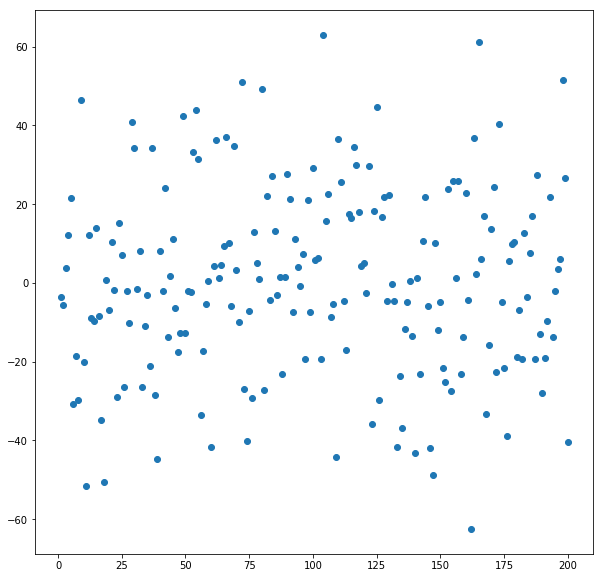
\includegraphics[width=\linewidth]{resid.png}

Для оценка нормальности остатков необходимо выполнить тест Харке-Бера.\newline
\begin{gather*}
    JB = (n-p-q-1)(\frac{\hat{S}^2}{6}-\frac{\hat{K}^2}{24})\\
    \hat{K} = \frac{\frac{1}{n}\sum_{i=1}^n(\varepsilon_i-\bar{\varepsilon})^4}{(\frac{1}{n-1}\sum_{i=1}^{n}(\varepsilon_i-\bar{\varepsilon})^2)^2}-3\\
    \hat{S} = \frac{\frac{1}{n}\sum_{i=1}^n(\varepsilon_i-\bar{\varepsilon})^3}{(\frac{1}{n-1}\sum_{i=1}^{n}(\varepsilon_i-\bar{\varepsilon})^2)^{\frac{3}{2}}}
\end{gather*}

Где $\hat{S}$ - выборочная ассиметричность, и $\hat{K}$ - выборочный экцесс.\newline
Проверить гипотезу $H_0: \{\varepsilon_t\}$ - i.i.d. ($K=3$, $S=0$) против альтернативной гипотезы $H_A: \{\varepsilon_t\}$ - не i.i.d. ($K\neq3$, $S\neq0$), с помощью $\chi^2$-статистики ($df=2$, $\alpha=0.05$), если $H_0$ не отвергается, то остатки нормальны.\newline

sample skew of the residuals is 0.066

sample kurtosis of the residuals is 2.739

Jarque-Bera statistic for AR(2) residuals: 0.7115

p-value: 0.7\newline

Т.е. на уровне значимости $\alpha=0.05$ гипотеза о нормальности остатков не отвергается. Отметим, что тест на Харке-Бера не необходим для прогнозирования, но для тестов Дики-Фулера используется предположение о нормальности остатков.\newpage

\section{Прогноз на один шаг}
\begin{gather*}
    X_t = \alpha_1X_{t-1}+\alpha_2X_{t-2} + \varepsilon_t\\
    X_{t+1}=E(X_{t+1}|X_{t})= E(\alpha_1X_{t}+\varepsilon_t|X_{t})+E(\alpha_2X_{t-1}+\varepsilon_{t-1}|X_{t-1})\\
    =\alpha_1X_{t}+\alpha_2X_{t-1}
\end{gather*}
По расчетам при $AR(2)$ модели:\newline

$\hat{X}_{200} = -5.951$; real $X_{200} = -46.334$

$\hat{X}_{199} = -33.203$;	real $X_{199} = -6.493$

$\hat{X}_{198} = -1.893$;	real $X_{198} = 49.608$

$\hat{X}_{197} = -3.620$;	real $X_{197} = 2.337$

$\hat{X}_{196} = -1.880$;	real $X_{196} = 1.702$
\end{document}
